\documentclass[aspectratio=169, 10pt]{beamer}

% ============================================================
% Lecture 3: Synthetic Control, RDD, and Shift-Share IV
% PhD programme: Economics, Management and Methods for the
% Sustainable Transition — University of Ferrara, 7 May 2026
% Author: Francesco Rentocchini
% Source material:
%   Abadie, Diamond & Hainmueller (2010); Cunningham (2021)
%   Cattaneo, Idrobo & Titiunik (2019); Calonico et al. (2014)
%   Borusyak, Hull & Jaravel (2022); Goldsmith-Pinkham et al. (2020)
% ============================================================

\usetheme{default}
% ============================================================
% preamble.tex — fit_phd_lectures
% Adapted from Scott Cunningham's Causal Inference Mixtape Sessions
% Compatible with pdflatex
% ============================================================

% --- Colors — JRC / European Commission identity ------------
\usepackage{xcolor}

% EC / JRC brand palette — softer pastel-leaning blue
\definecolor{ecblue}{HTML}{2E75B6}    % JRC pastel blue (softer than flag blue)
\definecolor{jrcblue}{HTML}{5B9BD5}   % JRC lighter accent blue
\definecolor{eugold}{HTML}{FFCC00}    % EU flag gold
\definecolor{ecnavy}{HTML}{1F3864}    % deep navy for text / headers
\definecolor{ecgray}{HTML}{54585A}    % EC institutional gray
\definecolor{ecred}{HTML}{C0392B}     % alert / warning red
\definecolor{ecgreen}{HTML}{1E7D34}   % example / positive green
\definecolor{lightblue}{HTML}{DEEBF7} % light blue tint for block bodies
\definecolor{offwhite}{HTML}{F7F8FC}  % near-white slide bg

% Convenience aliases
\definecolor{accent}{HTML}{2E75B6}    % = ecblue
\definecolor{accent2}{HTML}{C0392B}   % = ecred
\definecolor{gray100}{HTML}{DEEBF7}   % = lightblue
\definecolor{gray800}{HTML}{1F3864}   % = ecnavy

% Legacy aliases (used in slide source — map to JRC equivalents)
\definecolor{jet}{HTML}{1B2A6B}       % was near-black, now ecnavy
\definecolor{asher}{HTML}{54585A}     % was mid-gray, now ecgray
\definecolor{daisy}{HTML}{FFCC00}     % was yellow, now eugold
\definecolor{alice}{HTML}{0065A2}     % was teal, now jrcblue
\definecolor{coral}{HTML}{C0392B}     % was orange-red, now ecred
\definecolor{ruby}{HTML}{C0392B}      % was dark red, now ecred
\definecolor{kelly}{HTML}{1E7D34}     % was olive, now ecgreen
\definecolor{cranberry}{HTML}{C0392B} % was pink-red, now ecred

% --- Beamer theme — JRC style -------------------------------
\setbeamercolor{background canvas}{bg = white}
\setbeamersize{text margin left = 15pt, text margin right = 15pt}

% Frame title: white text on EC blue bar
\setbeamercolor{frametitle}{bg = ecblue, fg = white}
\setbeamercolor{framesubtitle}{bg = ecblue, fg = eugold}
\setbeamerfont{frametitle}{size = \normalsize, series = \bfseries}
\setbeamerfont{framesubtitle}{size = \small, shape = \itshape}

% Alerts
\setbeamercolor{alerted text}{fg = ecred}

% Blocks
\setbeamercolor{block title}{fg = white, bg = ecblue}
\setbeamercolor{block body}{fg = ecnavy, bg = lightblue}
\setbeamercolor{alertblock title}{fg = white, bg = ecred}
\setbeamercolor{alertblock body}{fg = ecnavy, bg = lightblue}
\setbeamercolor{exampleblock title}{fg = ecnavy, bg = eugold}
\setbeamercolor{exampleblock body}{fg = ecnavy, bg = lightblue}

% Title page — clean JRC style: white bg, left blue stripe, dark title text
% Slide canvas: 160mm × 90mm (aspectratio=169)
\setbeamercolor{title}{fg = ecnavy}
\setbeamercolor{subtitle}{fg = ecblue}
\setbeamerfont{title}{size = \LARGE, series = \bfseries}
\setbeamertemplate{title page}{%
    \begin{tikzpicture}[remember picture, overlay]
        % Left blue stripe (12mm wide, full height)
        \fill[ecblue] (current page.north west)
            rectangle ([xshift=12mm]current page.south west);
        % Gold horizontal accent line (~60% width, vertically centred below title)
        \draw[eugold, line width=2.5pt]
            ([xshift=16mm, yshift=-43mm]current page.north west) --
            ([xshift=150mm, yshift=-43mm]current page.north west);
        % Title — large, dark navy, on white area
        \node[anchor=north west, text width=136mm, align=left,
              font=\LARGE\bfseries, text=ecnavy]
            at ([xshift=16mm, yshift=-9mm]current page.north west)
            {\inserttitle};
        % Subtitle — below gold line, in pastel blue italic
        \node[anchor=north west, text width=136mm, align=left,
              font=\normalsize\itshape, text=ecblue]
            at ([xshift=16mm, yshift=-49mm]current page.north west)
            {\insertsubtitle};
        % Author — bold navy
        \node[anchor=north west, text width=136mm, align=left,
              font=\normalsize\bfseries, text=ecnavy]
            at ([xshift=16mm, yshift=-66mm]current page.north west)
            {\insertauthor};
        % Institution · date — small gray
        \node[anchor=north west, text width=136mm, align=left,
              font=\small, text=ecgray]
            at ([xshift=16mm, yshift=-74mm]current page.north west)
            {\insertinstitute\ \textbullet\ \insertdate};
    \end{tikzpicture}%
}

% TOC
\setbeamercolor{section in toc}{fg = ecblue}
\setbeamercolor{subsection in toc}{fg = ecnavy}

% Navigation
\setbeamertemplate{navigation symbols}{}

% Footer: thin gold line + institution name left, slide number right
\setbeamertemplate{footline}{%
    \begin{beamercolorbox}[wd=\paperwidth, ht=0.4pt]{frametitle}%
        \color{eugold}\rule{\paperwidth}{0.4pt}%
    \end{beamercolorbox}%
    \begin{beamercolorbox}[wd=\paperwidth, ht=5pt, dp=3pt,
            leftskip=6pt, rightskip=6pt]{normal text}%
        {\color{ecgray}\tiny F. Rentocchini / European Commission, JRC-Seville \& DEMM, University of Milan \hfill
         \color{ecgray}\tiny \ifnum\insertframenumber>1 \insertframenumber\fi}%
    \end{beamercolorbox}%
}

% Bullet points
\settowidth{\leftmargini}{\usebeamertemplate{itemize item}}
\addtolength{\leftmargini}{\labelsep}
\setbeamercolor{enumerate item}{fg = ecblue}
\setbeamertemplate{enumerate item}{\insertenumlabel.}
\setbeamercolor{itemize item}{fg = ecblue}
\setbeamertemplate{itemize item}[circle]
\setbeamercolor{itemize subitem}{fg = jrcblue}
\setbeamertemplate{itemize subitem}{$\rightarrow$}

% --- Section transition frames — EC blue bg, gold text ------
\newenvironment{transitionframe}{
    \setbeamercolor{background canvas}{bg = ecblue}
    \begin{frame}\color{white}\LARGE\centering
}{
    \end{frame}
}

% --- Auto-roadmap at each section ---------------------------
\AtBeginSection[]{
    \begin{frame}{Roadmap}
        \tableofcontents[currentsection]
    \end{frame}
}

% --- Packages -----------------------------------------------
\usepackage{amsmath, amssymb, amsthm}
\usepackage{graphicx}
\usepackage{booktabs}
\usepackage{array, adjustbox, tabularx}
\usepackage{threeparttable}
\usepackage{setspace}
\setstretch{1.15}
\usepackage{multicol}
\usepackage[protrusion=false,expansion=false]{microtype}
\usepackage{hyperref}
\hypersetup{colorlinks=true, linkcolor=accent2, urlcolor=accent2, citecolor=accent2}
\pdfstringdefDisableCommands{%
  \def\translate#1{#1}%
  \def\color#1{}%
}

% --- TikZ for DAGs ------------------------------------------
\usepackage{tikz}
\usetikzlibrary{positioning, arrows.meta, shapes.geometric, calc, fit}

% DAG style shortcuts
\tikzset{
    node/.style = {circle, draw=accent, fill=gray100, thick,
                   minimum size=8mm, font=\small},
    latent/.style = {circle, draw=accent, dashed, fill=white, thick,
                     minimum size=8mm, font=\small},
    arrow/.style = {-{Stealth[length=6pt]}, thick, color=jet},
    redarrow/.style = {-{Stealth[length=6pt]}, thick, color=accent2},
    bluearrow/.style = {-{Stealth[length=6pt]}, thick, color=accent},
}

% --- Highlighting box for equations -------------------------
\newcommand{\highlight}[1]{%
    \colorbox{eugold!50}{$\displaystyle #1$}}

% --- Fix \input with tables ---------------------------------
\makeatletter
\let\input\@@input
\makeatother

% Suppress overfull warnings
\vfuzz2pt
\hfuzz2pt


\usepackage{natbib}
\bibliographystyle{apalike}
\usepackage{colortbl}

% ---- Title --------------------------------------------------
\title[Synth, RDD, Shift-Share]{%
  Of Synthetic Realms, Discontinuities, and Shift-Shares}
\subtitle{Lecture 3: Synthetic Control, RDD, and Shift-Share\\
  {\small\normalfont\color{ecgray} PhD Economics, Management and Methods for the Sustainable Transition \textbullet\ University of Ferrara}}
\author{Francesco Rentocchini}
\institute{European Commission, JRC-Seville / DEMM, University of Milan}
\date{5-7 May 2026}

% ============================================================
\begin{document}
% ============================================================

\begin{frame}
  \titlepage
\end{frame}

\begin{frame}{Today's roadmap}
  \tableofcontents
\end{frame}

% ============================================================
\section{Synthetic Control}
% ============================================================

% --- Frame 1: Motivation ------------------------------------
\begin{frame}{The single-treated-unit problem}

  \begin{columns}[T]
    \begin{column}{0.52\textwidth}
      \textbf{When DiD breaks down}
      \begin{itemize}
        \item DiD needs many treated units for inference
        \item Policy often applies to \emph{one} state, country, or city
        \item Who is the right control group?
        \item Researcher discretion $\Rightarrow$ cherry-picking risk
      \end{itemize}

      \bigskip
      \textbf{The question \citep{abadie2010}}\\[2pt]
      California passes Proposition~99 in 1988: a large tobacco tax.
      \emph{What would cigarette consumption have been without it?}

      \medskip
      \begin{alertblock}{The challenge}
        No single state is a good control. Using all states or a
        researcher-chosen subset gives different answers.
      \end{alertblock}
    \end{column}
    \begin{column}{0.44\textwidth}
      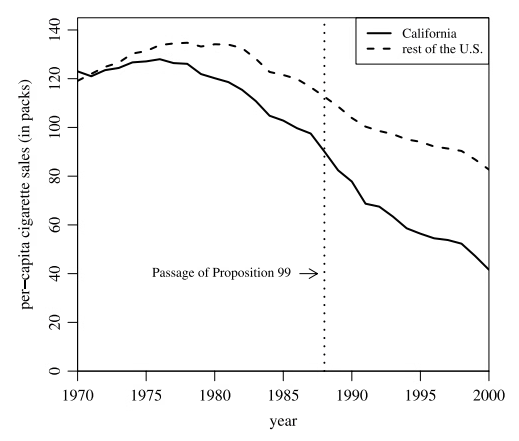
\includegraphics[width=\linewidth]{../Figures/L3_abadie1.png}
      \smallskip\small
      \textbf{Why not "rest of US"?}
      The naive control (dashed) trends \emph{upward} while CA
      declines pre-1988 — parallel trends fails.
    \end{column}
  \end{columns}

\end{frame}

% --- Frame 2: The method ------------------------------------
\begin{frame}[shrink=5]{Synthetic Control: building the counterfactual}

  \begin{columns}[T]
    \begin{column}{0.50\textwidth}
      \textbf{Setup} \citep{abadie2010}
      \begin{itemize}
        \item $J+1$ units, $T$ periods; unit~1 treated at $T_0$
        \item \emph{Donor pool}: units $2,\ldots,J+1$ never treated
        \item \emph{Synthetic control}:
          $\hat{Y}_{1t}^{(0)} = \textstyle\sum_{j=2}^{J+1} w_j^{\,*}\, Y_{jt}$
        \item Weights: $w_j^* \geq 0$, $\textstyle\sum w_j^* = 1$
      \end{itemize}

      \smallskip
      \textbf{How weights are chosen}\\
      Minimise pre-treatment prediction error:
      \[
        W^* = \arg\min_W \; \|X_1 - X_0 W\|_V
      \]
      $X_1, X_0$: outcome lags + covariates; $V$: importance matrix.

      \smallskip
      \begin{block}{Key property}\small
        $w_j^* \geq 0$, $\sum w_j^* = 1$ $\Rightarrow$ interpolation only;
        no extrapolation outside the convex hull of donors.
      \end{block}
    \end{column}
    \begin{column}{0.46\textwidth}
      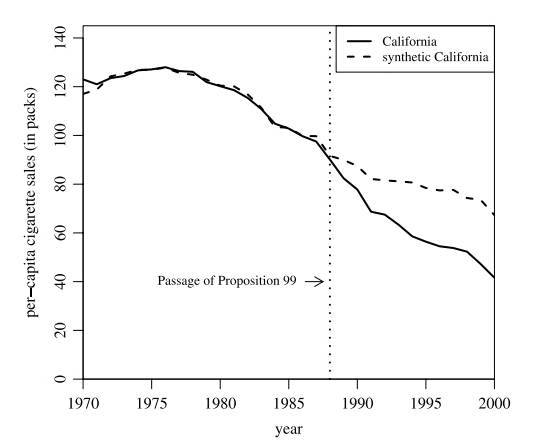
\includegraphics[width=0.93\linewidth]{../Figures/L3_abadie.png}

      \smallskip\scriptsize\centering
      CA vs synthetic CA, 1970--2000: tight pre-fit,
      sharp post-1988 divergence = treatment effect.

      \smallskip\raggedright
      \textbf{Sparse weights:} CT\,(0.69), CO\,(0.16),
      NV\,(0.09), MT\,(0.05), UT\,(0.01)\\
      Pre-fit RMSPE: synth\,$\approx$1.6 vs rest-of-US\,$\approx$8.0 packs.
    \end{column}
  \end{columns}

\end{frame}

% --- Frame 3: Inference -------------------------------------
\begin{frame}{Inference: the placebo (permutation) test \citep{abadie2010}}

  \begin{columns}[T]
    \begin{column}{0.50\textwidth}
      \textbf{Why standard errors fail}\\\small
      One treated unit $\Rightarrow$ no asymptotic distribution.
      Standard bootstrapping and DiD SEs both require many units.

      \smallskip
      \textbf{Placebo logic} \citep{abadie2010}: apply synth to
      \textbf{each donor state} as if treated in 1988, then rank
      states by the post/pre RMSPE ratio:
      \[
        r_j = \frac{\text{RMSPE}_{\text{post}}}{\text{RMSPE}_{\text{pre}}}
      \]
      Dividing by pre-RMSPE controls for poor pre-fit.\\
      \textbf{p-value} = share of states with $r_j \geq r_{\text{CA}}$.

      \begin{block}{Result}\small
        CA ranks \textbf{1st out of 39 states}:
        $p = 1/39 \approx 0.026$.
      \end{block}
    \end{column}
    \begin{column}{0.46\textwidth}
      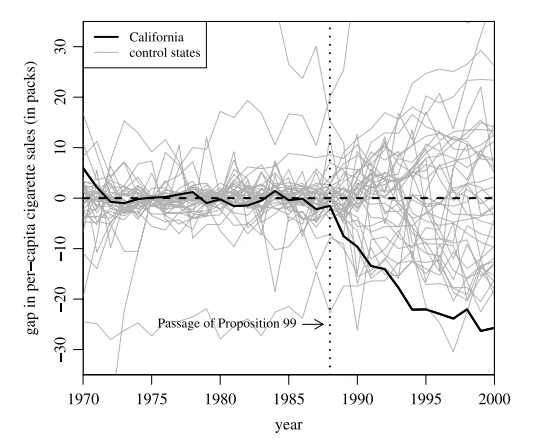
\includegraphics[width=\linewidth]{../Figures/L3_abadie2.png}

      \smallskip\scriptsize
      Gray: gap (actual $-$ synthetic) for each placebo state.
      Black: California. Pre-1988 all gaps cluster near zero;
      post-1988 CA drops to $-$26 packs — far below every placebo.
      That is the visual $p$-value.
    \end{column}
  \end{columns}

\end{frame}

% --- Frame 4: Limitations -----------------------------------
\begin{frame}[shrink=5]{Synthetic Control: when it works — and when it doesn't}

  \begin{columns}[T]
    \begin{column}{0.48\textwidth}
      \begin{block}{When synth works well}
        \begin{itemize}
          \item Aggregate-level treatment (state, country, city)
          \item Long pre-treatment period ($T_0 \geq 10$ periods)
          \item Good pre-treatment fit available from donor pool
          \item Single or few treated units
          \item Policy well-defined with known timing
        \end{itemize}
      \end{block}
    \end{column}
    \begin{column}{0.48\textwidth}
      \begin{alertblock}{When synth fails}
        \begin{itemize}
          \item No good match in donor pool (large pre-RMSPE)
          \item Donor units also partially treated or anticipate treatment
          \item Short pre-period $\Rightarrow$ over-fit
          \item Spillovers from treated to donors
        \end{itemize}
      \end{alertblock}
    \end{column}
  \end{columns}

  \medskip
      \textbf{Synth vs.\ DiD — the key trade-off}
      \begin{itemize}\small
        \item DiD requires \textbf{parallel trends}
        \item Synth replaces this with \textbf{convex hull inclusion}:
              the treated unit's pre-treatment path must lie in the
              convex hull of the donor pool $\Rightarrow$ \emph{less stringent}
        \item If the treated unit is an outlier that no weighted
              combination of donors can reproduce, pre-fit will be
              poor and the estimate invalid
      \end{itemize}


\end{frame}




% --- Frame 6: Synthetic DiD extension -------------------------
\begin{frame}[shrink=10]{Extension: Synthetic Difference-in-Differences}

  \begin{columns}[T]
    \begin{column}{0.50\textwidth}
      \textbf{Bridging Synth and DiD} \citep{arkhangelsky2021}\\[4pt]
      Both methods share a flaw:
      \begin{itemize}
        \item DiD: parallel trends may not hold
        \item Synth: treated unit must lie in the convex hull of donors
      \end{itemize}

      \medskip
      \textbf{SDID solves both by combining}
      \begin{itemize}
        \item \emph{Unit weights} $\hat\omega_j$ — like synthetic control,
              re-weight donors to match treated pre-trends
        \item \emph{Time weights} $\hat\lambda_t$ — up-weight
              pre-treatment periods that look most like the treatment period
      \end{itemize}

      \medskip
      \textbf{Estimator}
      \[
        \hat\tau^{\text{SDID}} =
        \arg\min_{\tau,\alpha,\beta}\,
        \sum_{i,t} \hat\omega_i\,\hat\lambda_t
        \bigl(Y_{it} - \alpha_i - \beta_t - \tau D_{it}\bigr)^2
      \]
    \end{column}
    \begin{column}{0.46\textwidth}
      \begin{block}{Key properties}
        \begin{itemize}\small
          \item Consistent even if trends are \emph{not} parallel
          \item Works with multiple treated units (unlike basic synth)
          \item Nests DiD ($\hat\omega_j = 1/N_{\text{ctrl}}$) and SC
                ($\hat\lambda_t = 1/T_{\text{pre}}$)
          \item Bootstrap/placebo inference
        \end{itemize}
      \end{block}

      \medskip
      \begin{exampleblock}{When to prefer SDID over Synth}
        \small Many treated units; possible pre-trend divergence;
        want standard errors with a formula (not just permutation).
      \end{exampleblock}
    \end{column}
  \end{columns}

\end{frame}


% ============================================================
\section{Regression Discontinuity Design}
% ============================================================

% --- Frame 5: The design ------------------------------------
\begin{frame}{Sharp RDD: threshold and local randomisation}

      \textbf{The design}
      \begin{itemize}
        \item Running variable $X_i$ (score, vote margin, \ldots)
        \item Threshold $c$: $D_i = \mathbf{1}[X_i \geq c]$
        \item Units near $c$ are locally comparable
        \item Assignment ``as good as random'' near cutoff
      \end{itemize}

\end{frame}

% --- Frame 5b: Santoleri et al. (2024) RDD application -------
\begin{frame}[shrink=5]{Application: causal effects of R\&D grants \citep{santoleri2024}}

  \begin{columns}[T]
    \begin{column}{0.50\textwidth}
      \textbf{Design}
      \begin{itemize}\small
        \item \textbf{Programme:} EU SME Instrument (Horizon 2020)
              — first European R\&D grant targeting small innovative
              firms; grants up to \texteuro2.5m
        \item \textbf{Running variable:} expert panel score rank
              (centered at funding threshold)
        \item \textbf{Treatment:} grant awarded ($\text{rank} \geq 0$)
        \item \textbf{Sample:} firms from $>$40 countries, virtually
              all sectors
      \end{itemize}

      \smallskip
      \begin{block}{Key results}\small
        \begin{itemize}
          \item \textbf{+15\%--31\%} cite-weighted patents
                (intensive \& extensive margins)
          \item \textbf{$>$100\%} increase in probability of
                receiving follow-on private equity
          \item Effects larger for younger, smaller firms and
                financially constrained sectors/regions
        \end{itemize}
      \end{block}

      \smallskip
      \begin{exampleblock}{Mechanism: funding $\gg$ certification}\small
        Firms receiving only a ``quality stamp'' (no money)
        do \textbf{not} improve — direct causal evidence that
        the grant's value is the \emph{funding}, not the signal.
      \end{exampleblock}
    \end{column}
    \begin{column}{0.46\textwidth}
      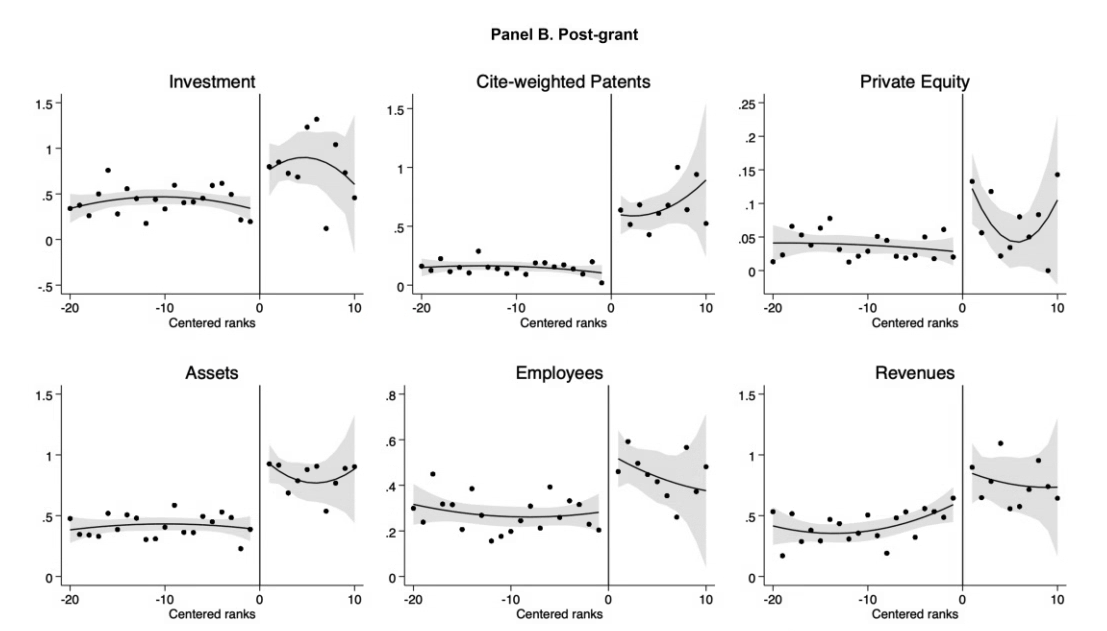
\includegraphics[width=\linewidth]{../Figures/L3_santoleri.png}

      \smallskip\scriptsize
      Panel B (post-grant): RD plots at the funding threshold
      (centered rank\,$=0$). Clear jumps for investment,
      cite-weighted patents, and private equity. Threshold
      assignment identifies the causal effect.
    \end{column}
  \end{columns}

\end{frame}

% --- Frame 6: Identification ---------------------------------
\begin{frame}[shrink=5]{Identification: the continuity assumption}

  \begin{columns}[T]
    \begin{column}{0.52\textwidth}
      \textbf{Formal assumption}\\[4pt]
      The potential outcome functions
      \[
        E\!\left[Y_i^{(0)}\mid X_i=x\right] \text{ and }
        E\!\left[Y_i^{(1)}\mid X_i=x\right]
      \]
      are \textbf{continuous} in $x$ at $c$.

      \smallskip
      \textbf{What this buys}
      \[
        \hat\tau_{\text{RDD}} =
        \lim_{x\downarrow c} E[Y\mid X=x]
        - \lim_{x\uparrow c} E[Y\mid X=x]
      \]
      Identifies the \textbf{Local Average Treatment Effect at $c$}.

      \smallskip
      \textbf{What it doesn't}
      \begin{itemize}
        \item LATE $\neq$ ATE (effect may vary away from threshold)
        \item Cannot extrapolate away from $c$
        \item Says nothing about why the discontinuity holds
      \end{itemize}
    \end{column}
    \begin{column}{0.44\textwidth}
      \begin{alertblock}{Key violation: manipulation}\small
        If units sort above/below $c$, $X_i$ is not continuously
        distributed there. Examples: students repeating exams,
        parties inflating vote counts, firms manipulating ratios.
      \end{alertblock}

      \smallskip
      \begin{block}{Local vs.\ global}
        \small RDD is \emph{local}: only observations near $c$ identify
        $\tau$. This is a feature (credibility) and a limitation
        (external validity).
      \end{block}
    \end{column}
  \end{columns}

\end{frame}

% --- Frame 7a: rdplot decisions ------------------------------
\begin{frame}[shrink=5]{RD plots: key decisions \citep{cattaneo2019}}

  \begin{columns}[T]
    \begin{column}{0.50\textwidth}
      \small Visualise the jump at the cutoff. The plot uses
      \emph{binned sample means} (dots) plus a \emph{global polynomial
      smooth} (line) separately on each side.

      \medskip
      \textbf{Decision 1 — Bin type}
      \begin{itemize}\small
        \item \textbf{Evenly-spaced (ES):} bins of equal width.
              Works well when the score is roughly uniform.
        \item \textbf{Quantile-spaced (QS):} bins with equal
              \emph{number of observations}. Better when the score
              is skewed or uneven — avoids bins with very few points.
      \end{itemize}

      \smallskip
      \textbf{Decision 2 — Number of bins}
      \begin{itemize}\small
        \item \textbf{IMSE-optimal:} smooth plot showing overall regression shape. 
        \item \textbf{MV (mimicking variance):} more bins $\rightarrow$ to see scatter around the trend near the cutoff.
      \end{itemize}
    \end{column}
    \begin{column}{0.46\textwidth}
      \textbf{Decision 3 — Global polynomial order}\\[3pt]
      \small The smooth line uses a \emph{global} polynomial (default
      order 4) to illustrate the overall shape $\rightarrow$ for
      \emph{visualisation only}, not for the formal estimate.

      \smallskip
      \begin{block}{Recommended default: QS\,+\,MV}\small
        Quantile-spaced bins + MV number of bins shows the local
        variability and handles uneven score distributions. $\rightarrow$ can switch to IMSE to assess
        the global shape of the regression function.
      \end{block}

      \smallskip\small
      \textbf{What to look for:} a clear jump in the binned means at
      $c$. If dots on the two sides overlap near $c$ $\rightarrow$ effect small or absent.
    \end{column}
  \end{columns}

\end{frame}

% --- Frame 7b: Estimation — estimator, polynomial, kernel, bandwidth ---
\begin{frame}[shrink=5]{Estimation: key decisions (1--3) \citep{cattaneo2019}}

  \begin{columns}[T]
    \begin{column}{0.50\textwidth}
      \textbf{The local linear estimator ($p=1$)}\\[2pt]
      Within bandwidth $h$ on each side of $c$, fit:
      \[
        Y_i = \alpha + \tau D_i + \beta(X_i - c) + \gamma D_i(X_i - c) + \varepsilon_i
      \]
%      with kernel weights $K\!\left(\tfrac{X_i-c}{h}\right)$.
      The intercept jump $\hat\tau$ is the RD estimate.

      \smallskip
      \textbf{Decision 1 — Polynomial order $p$}
      \begin{itemize}
        \item \textbf{Local linear ($p=1$):} \emph{recommended default}.
              Robust to boundary problems; no overfitting.
        \item \textbf{Local quadratic ($p=2$):} used for
              bias-correction only (no estimate).
        \item \textbf{Global polynomials:} never use $\rightarrow$ poor at boundaries; misleading results.
      \end{itemize}
    \end{column}
    \begin{column}{0.46\textwidth}
      \textbf{Decision 2 — Kernel function $K(\cdot)$}
      \begin{itemize}
        \item \textbf{Triangular:} more weight
              to observations closer to $c$. \emph{Recommended}
        \item \textbf{Uniform:} equal weights $\rightarrow$ only with very few observations near the cutoff.
      \end{itemize}

      \smallskip
      \textbf{Decision 3 — Bandwidth $h$}
      \begin{itemize}
        \item \textbf{MSE-optimal \citep{calonico2014}:}
              balances bias and variance. \emph{Use for point
              estimation.}
        \item \textbf{CER-optimal:} smaller bandwidth that minimises
              coverage error of confidence intervals. \emph{Use for
              inference} when coverage accuracy matters most.
        \item \textbf{Two bandwidths} ($h_-$, $h_+$): allowed when
              curvature or density differs across sides.
      \end{itemize}
    \end{column}
  \end{columns}

\end{frame}

% --- Frame 7c: Estimation — inference, covariates, clustering ---
\begin{frame}[shrink=5]{Estimation: key decisions (4--6) \citep{cattaneo2019}}


      \textbf{Decision 4 — Inference: bias-correction and robust CIs}
      \begin{itemize}
        \item point estimator has
              \emph{non-negligible bias} $\Rightarrow$ CIs are incorrect $\rightarrow$ \citet{calonico2014}:
              estimate the bias using a local polynomial of
              order $p+1$ and subtract it
      \end{itemize}

      \smallskip
      \textbf{Decision 5 — Predetermined covariates}
      \begin{itemize}
        \item Including covariates only improves \emph{precision}
              by reducing residual variance.
        \item Only use \textbf{pre-determined} covariates
        \item Check: covariates should show \emph{no jump} at $c$
              (balance test); if they do, the RD assumption fails.
      \end{itemize}

      \smallskip
      \textbf{Decision 6 — Clustering}
      \begin{itemize}
        \item Cluster if observations within a group share common
              unobservables (e.g., same school, district, year).
      \end{itemize}
\bigskip
      \begin{block}{Rule of thumb}
        $p=1$ + triangular kernel + MSE bandwidth + robust CI.
        Always report bandwidth sensitivity.
      \end{block}


\end{frame}

% --- Frame 8: Validity tests ---------------------------------
\begin{frame}[shrink=15]{Validity: what you must always check}

  \begin{columns}[T]
    \begin{column}{0.48\textwidth}
      \begin{block}{1.\ Density test}
        Is the density of $X_i$ continuous at $c$? \\
        A jump $\Rightarrow$ units are sorting; running variable is
        manipulated. \emph{E.g.\ firms inflating R\&D spend just above the
        eligibility threshold to qualify for a grant.}
      \end{block}

      \smallskip
      \begin{block}{2.\ Covariate balance}
        Run RDD on pre-determined covariates.\\
        Should find \textbf{no jump} at $c$.
      \end{block}

      \smallskip
      \begin{block}{3.\ Placebo outcomes \citep{cattaneo2019}}
        \small Outcomes measured \emph{after} treatment but causally
        unrelated to it — should find \textbf{no effect}.\\
        \emph{Clean water: car accident mortality is a valid placebo;
        water-borne illness mortality is not.}
      \end{block}
    \end{column}
    \begin{column}{0.48\textwidth}
      \begin{block}{4.\ Placebo cutoffs}
        Test at arbitrary thresholds $c' \neq c$ within the support.\\
        Should find \textbf{no significant effect}
      \end{block}

      \smallskip
      \begin{block}{5.\ Bandwidth sensitivity}
        Plot $\hat\tau(h)$ for a range of bandwidths.\\
        Stable $\Rightarrow$ reassuring
      \end{block}

      \smallskip
      \begin{block}{6.\ Donut RDD}
        Exclude obs.\ within a small radius $\delta$ of $c$.\\
        Tests whether the effect is driven by near-threshold
        manipulation. Effect should persist with $\delta>0$.
      \end{block}
    \end{column}
  \end{columns}

\end{frame}


% ============================================================
\section{Shift-Share IV}
% ============================================================

% --- Frame 9: What is SSIV ----------------------------------
\begin{frame}[shrink=9]{The shift-share instrument}

  \begin{columns}[T]
    \begin{column}{0.50\textwidth}
      \[
        z_\ell = \sum_{n=1}^{N} \underbrace{s_{\ell n}}_{\text{shares}}
                 \cdot \underbrace{g_n}_{\text{shocks}}
      \]
      \begin{itemize}\small
        \item $s_{\ell n}$: lagged employment share of industry $n$ in region $\ell$
        \item $g_n$: national (leave-one-out) employment growth in industry $n$
        \item $z_\ell$: predicted local employment growth from national trends
      \end{itemize}
    \end{column}
    \begin{column}{0.46\textwidth}
      \textbf{Idea \citep{bartik1991}}\\
      \small Two regions with different industry mixes receive
      \emph{different shocks} even if the national trend is the same —
      generating exogenous variation in the endogenous treatment.

      \smallskip
      \begin{block}{\small Notation}
        \small Model: $y_\ell = \beta x_\ell + \gamma' w_\ell + \varepsilon_\ell$\\
        Use $z_\ell$ as IV for the endogenous $x_\ell$.\\
        Validity: $E[z_\ell \varepsilon_\ell] = 0$
      \end{block}
    \end{column}
  \end{columns}

  \smallskip
  \textbf{Three canonical applications}

  \smallskip
  {\scriptsize\renewcommand{\arraystretch}{1.2}%
  \begin{tabularx}{\linewidth}{l>{\raggedright\arraybackslash}X>{\raggedright\arraybackslash}X>{\raggedright\arraybackslash}X>{\raggedright\arraybackslash}X}
    \toprule
    Paper & Shares $s_{\ell n}$ & Shocks $g_n$ & Outcome $y_\ell$ & Data level \\
    \midrule
    Bartik (1991) & Lagged industry empl.\ shares & Natl.\ empl.\ growth by industry & Local employment growth & MSAs \\
    ADH (2013)    & Mfg.\ empl.\ shares (10-yr lag) & China exports to 8 non-US countries & Mfg.\ employment \& wages & Commuting zones \\
    Card (2009)   & Migrant enclaves (past shares) & Natl.\ immigration by origin & Native wages by education & Cities/MSAs \\
    \bottomrule
  \end{tabularx}}

\end{frame}

% --- Frame 10: Two identification strategies ----------------
\begin{frame}[shrink=5]{Two ways to justify SSIV}

  \begin{columns}[T]
    \begin{column}{0.48\textwidth}
      \begin{block}{Strategy 1: Shock exogeneity (BHJ)}\small
        \citet{borusyak2022}: exogeneity lives in \textbf{shocks} $g_n$.

        \smallskip
        \textbf{Assumption:} $g_n$ quasi-randomly assigned across
        industries, conditional on controls.

        \smallskip
        \textbf{Implication:} shares $s_{\ell n}$ are just
        \emph{exposure weights} — need not be exogenous.

        \smallskip
        \textbf{Test:} pre-trend balance at the industry level.\\
        \textbf{Inference:} cluster at the industry (shock) level.
      \end{block}
    \end{column}
    \begin{column}{0.48\textwidth}
      \begin{block}{Strategy 2: Share exogeneity (GPSS)}\small
        \citet{goldsmithpinkham2020}: exogeneity lives in
        \textbf{shares} $s_{\ell n}$.

        \smallskip
        \textbf{Assumption:} $s_{\ell n}$ pre-determined and
        uncorrelated with $\varepsilon_\ell$.

        \smallskip
        \textbf{Implication:} SSIV = weighted avg of
        industry IVs with Rotemberg weights $\alpha_n$:
        \[
          \hat\beta = \textstyle\sum_n \alpha_n\, \hat\beta_n
        \]

        \textbf{Test:} shares uncorrelated with pre-trends?
        Rotemberg weights non-negative?
      \end{block}
    \end{column}
  \end{columns}

  \smallskip
  \begin{alertblock}{Two views — one instrument}\small
    Which view you take determines what you must defend.
    BHJ: many quasi-random shocks.
    GPSS: clean historical shares.
    Both require the exclusion restriction.
  \end{alertblock}

\end{frame}


% --- Frame 12: Practical considerations ---------------------
\begin{frame}[shrink=8]{SSIV in practice: checks by identification strategy}

  \begin{columns}[T]
    \begin{column}{0.48\textwidth}
      \begin{block}{Shock exogeneity (BHJ) — three checks}\small
        \textbf{1.\ Leave-one-out shocks}\\
        Exclude focal region from its own shock to avoid mechanical
        correlation:
        \[
          g_n^{(-\ell)} = \frac{\Delta E_n - \Delta E_{\ell n}}{E_n - E_{\ell n}}
        \]

        \textbf{2.\ Cluster at industry level}\\
        SEs must account for shock-level correlation \citep{adao2019}.
        Industries induce correlated residuals across regions with
        similar shares — cluster at the shock, not the region.

        \smallskip
        \textbf{3.\ Industry-level balance test}\\
        Regress $g_n$ on pre-determined industry characteristics.
        Significant predictors $\Rightarrow$ shocks not quasi-randomly
        assigned.
      \end{block}
    \end{column}
    \begin{column}{0.48\textwidth}
      \begin{block}{Share exogeneity (GPSS) — three checks}\small
        \textbf{1.\ Share pre-trends}\\
        For the highest-$\alpha_n$ industries, test whether $s_{\ell n}$
        predicts the outcome \emph{before} treatment.
        Significant pre-trends $\Rightarrow$ shares not pre-determined.

        \smallskip
        \textbf{2.\ Rotemberg weights}\\
        Compute $\alpha_n$ (each industry's contribution to $\hat\beta$).\\
        Check: (a) all $\alpha_n \geq 0$ — negative weights signal
        fragility; (b) no single industry dominates — concentration
        means the result rests on one sector's exogeneity (Drop top 3 industries; re-estimate. Stable $\rightarrow$ robust. Flips $\rightarrow$ fragile).

        \smallskip
        \textbf{3.\ Incomplete shares}\\
        If $\sum_n s_{\ell n} < 1$ (e.g.\ only manufacturing covered):
        normalise to sum to 1, or control for coverage share.
      \end{block}
    \end{column}
  \end{columns}

\end{frame}


% ============================================================
\section{Lab Preview}
% ============================================================



% --- Frame 5a: Pinotti — treatment: mafia expansion ----------
\begin{frame}[shrink=15]{Exercise 1: mafia expands into Apulia \& Basilicata \citep{pinotti2015}}

  \begin{columns}[T]
    \begin{column}{0.55\textwidth}
      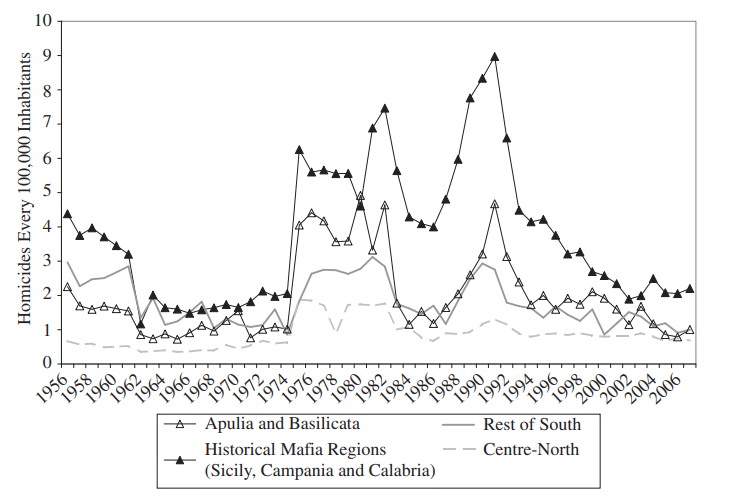
\includegraphics[width=\linewidth]{../Figures/L3_pinotti1.png}
    \end{column}
    \begin{column}{0.45\textwidth}
      \textbf{Research question:} causal economic cost of organised crime?

      \smallskip\small
      \textbf{Two exogenous drivers:}
      \begin{enumerate}\small
        \item \textbf{Tobacco route shift:} Tangier port closure
              (1960) $\Rightarrow$ depots move to E.\ Europe $\Rightarrow$
              syndicates switch from \emph{Tyrrhenian} (Morocco--Naples)
              to \emph{Adriatic route} (Albania--Apulia).
              Cigarette smuggling was the dominant criminal
              business of the 1970s.
        \item \textbf{Confino:} convicted mafia members forcibly
              relocated by government; Basilicata had the most
              in Italy (1961--72).
      \end{enumerate}

      \begin{block}{Why this matters for synth}\small
        Onset \textbf{dated} (homicides spike from 1975),
        \textbf{abrupt}, and \textbf{exogenous} — driven by
        port policy and geography, not regional choice.
      \end{block}
    \end{column}
  \end{columns}

\end{frame}

% --- Frame 5b: Pinotti — synthetic control result -------------
\begin{frame}[shrink=5]{Application: the economic cost of organised crime \citep{pinotti2015}}

  \begin{columns}[T]
    \begin{column}{0.50\textwidth}
      \textbf{Setup}
      \begin{itemize}\small
        \item \textbf{Treated:} Apulia \& Basilicata — free of mafia until
              rapid expansion in the early 1970s
        \item \textbf{Donor pool:} other Italian regions without mafia
        \item \textbf{Outcome:} GDP per capita (constant 1990 euros)
        \item \textbf{Pre-period:} post-war to early 1960s
              (matching period)
      \end{itemize}

      \smallskip
      \begin{block}{Why synth fits \& key result}\small
        \begin{itemize}
          \item Dated treatment onset, long clean pre-period
          \item $N_{\text{treated}}=2$ — too small for DiD inference
          \item Donor units unaffected by the same shock
          \item Mafia $\Rightarrow$ \textbf{$-16\%$ GDP per capita}.
                Mechanism: private investment crowded out by less
                productive public spending
        \end{itemize}
      \end{block}
    \end{column}

    \begin{column}{0.46\textwidth}
      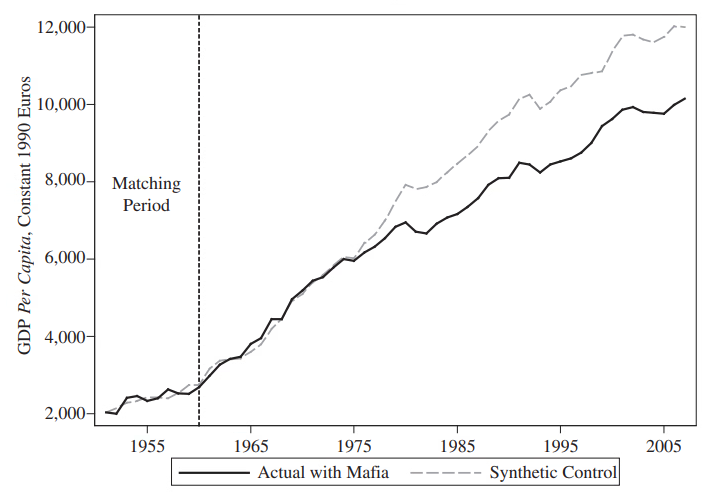
\includegraphics[width=\linewidth]{../Figures/L3_pinotti2.png}
    \end{column}
  \end{columns}

\end{frame}

\begin{frame}[shrink=15]{Exercise 2: Turkish municipal elections and female higher education completion rate \citep{meyersson2014}}

  \begin{columns}[T]
    \begin{column}{0.5\textwidth}
      \begin{itemize}
        \item  1994 Turkish municipal elections, $n \approx 2{,}629$
        \item Running var: Islamic party vote \emph{margin}.
        \item Treatment: Islamic mayor elected ($X_i \geq 0$).
        \item Outcome: female HS completion rate (2000).
        \item \textbf{Finding:} +4.4~pp for women in Islamic-won municipalities.

      \end{itemize}


    \end{column}
    \begin{column}{0.5\textwidth}
      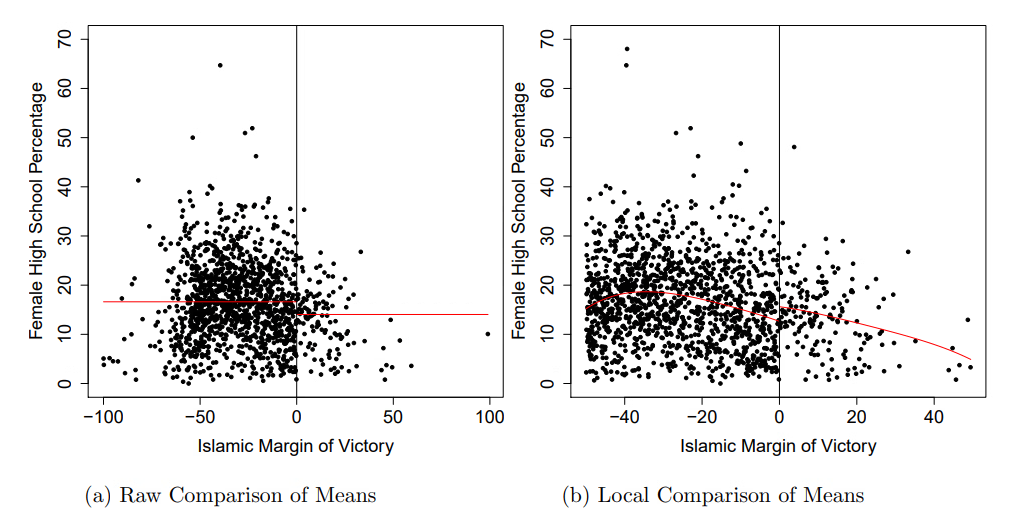
\includegraphics[width=\linewidth]{../Figures/L3_meyersson.png}

      \smallskip\scriptsize
      \textbf{(a)} Full bandwidth: no jump visible.
      \textbf{(b)} Local bandwidth: clear discontinuity at $c=0$.
    \end{column}

  \end{columns}
  \smallskip
  \begin{block}{Why does an Islamic mayor increase female HS completion? — main channels}\small
    \textbf{(1) Supply:} more schools built $\Rightarrow$ shorter travel distance, a binding constraint for girls in conservative households \hfill \\
    \textbf{(2) Legitimacy:} conservative families more willing to allow daughters to attend under a religiously aligned government \hfill \\
    \textbf{(3) Safety:} reduced social barriers (harassment, stigma) for girls commuting. \hfill \\
    \textbf{(4)} Effect is largest in poorer, more conservative areas $\rightarrow$ consistent with supply + social-norms channels.

  \end{block}

\end{frame}


\begin{frame}[shrink=15]{Exercise 3: the China shock and US manufacturing employment \citep{autor2013}}

  \begin{columns}[T]
    \begin{column}{0.50\textwidth}
      \begin{itemize}\small
        \item 722 US commuting zones, two decades (1990s, 2000s)
        \item \textbf{Endogenous:} $\Delta$ Chinese imports/worker ($x_\ell$)
        \item \textbf{Instrument:} $z_\ell = \sum_n s_{\ell n}^{\text{lag}} \cdot g_n^{\text{other}}$ — lagged CZ industry shares $\times$ China exports to 8 other countries
        \item \textbf{Outcome:} $\Delta$ manufacturing employment share
        \item \textbf{Finding:} \$1{,}000 more imports/worker $\Rightarrow -0.6$~pp mfg employment
      \end{itemize}

      \smallskip
      \begin{block}{Why the IV works}\small
        \begin{itemize}
          \item CZs with different industry mixes are hit differently by the same global shock.
          \item China exports to \emph{other} countries are exogenous to US local conditions.
          \item 2SLS $\gg$ OLS $\Rightarrow$ OLS is biased toward zero by two forces:
          \begin{itemize}
            \item \textbf{Measurement error:} industry misclassification in US customs data adds noise to $x_\ell$ $\Rightarrow$ attenuation
            \item \textbf{Simultaneity:} structurally declining regions attract cheap imports $\Rightarrow$ reverse causality also shrinks the OLS estimate
          \end{itemize}
        \end{itemize}
      \end{block}
    \end{column}

    \begin{column}{0.46\textwidth}
      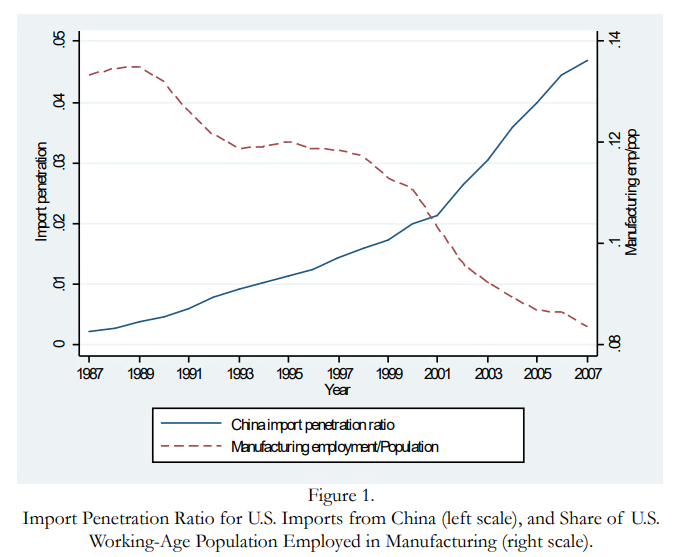
\includegraphics[width=\linewidth]{../Figures/L3_ADH.png}
    \end{column}
  \end{columns}

\end{frame}

% ============================================================
% References
% ============================================================

\begin{frame}[allowframebreaks]{References}
  \bibliography{../Bibliography_base}
\end{frame}

\end{document}
